\chapter{基于Kagome晶格的声学哈密顿量推导及边界条件对拓扑态的影响研究}

\section{引言}

一般来说,在量子系统中,真空可被视为围绕开放边界的非平凡结构的平凡域。然而,对于经典波系统(即声学系统)中类似的拓扑晶态绝缘体(TCIs),是我们施加的诸如硬边界或软边界等边界条件来构建有限结构,并且在这些边界上新兴态的自然行为是不同的。另一方面,与现有的专注于研究“零能”模式的理论模型不同,在实际物理系统中,相应哈密顿量的对角项(代表“虚拟”原子的在位能)总是不可忽略的。由于粒子-空穴对称性,体晶格中的这些项总是相同的;然而,有限结构边界上对称性的降低直接导致边界晶格上额外的跳跃,进而直接影响相应的在位项。因此,在位项如何影响哈密顿量,即边界对经典波系统中拓扑态产生的实际影响是什么,仍然是一个有待解决的问题。

本章工作的目的是通过实现声学和电子系统的类比,构造高阶拓扑绝缘体,并说明声学系统中独有的边界条件对拓扑态的影响。我们首先以Kagome晶格为例,在亚波长尺度下,讨论了声学系统和电子系统的相似性,在声学腔管模型中构造了Kagome晶格。然后,我们从声电类比方法出发,以前述章节的传统声学的角度严格推导出具有二维Kagome晶格的共振系统的哈密顿量,从而揭示理论模型中的晶胞内或晶胞间跳跃与实际物理系统中声学参数之间的联系。其中的关键是我们通过呈现一个有限时间反演不变拓扑结构,证明了不同边界条件对应于边缘晶格中不同的在位能。在这个模型里,除了非平庸拓扑相之外,拓扑态的在带隙内存在还要求哈密顿量对角项在体,边,角晶格上一致,因此系统的边界应为软边界。所有的理论预测都得到了使用有限元方法的数值模拟的精确支持。这些结果不仅揭示了从凝聚态物理中的拓扑绝缘体到声学系统的严格类比,还为设计具有任意期望频率拓扑态的声学拓扑系统提供了一个平台。

本章的主要内容如下:先在3.2节通过Kagome晶格与声学结构的类比,探寻两者间的相似性,为后续研究奠定基础。接着,3.3节推导Kagome晶格的声学哈密顿量,这一关键理论工具将助力我们深入理解其声学拓扑性质。而后,3.4节剖析无限大周期排列的Kagome晶格的拓扑相变,揭示其在不同参数下拓扑性质的变化规律与机制,为有限结构研究提供参考。3.5节聚焦有限大带状排列的Kagome晶格的拓扑态,探究其存在形式、分布特点及与边界条件的关联,以及有限尺寸效应对其的影响和调控方式。最后,3.6节研究有限大三角排列的Kagome晶格的拓扑态,分析其独特几何结构下拓扑态的特性、与带状排列的异同以及稳定性和可调控性。最后3.7节是本章的小结。


\section{Kagome晶格与声学结构类比}

\begin{figure}[h!]
  \centering
  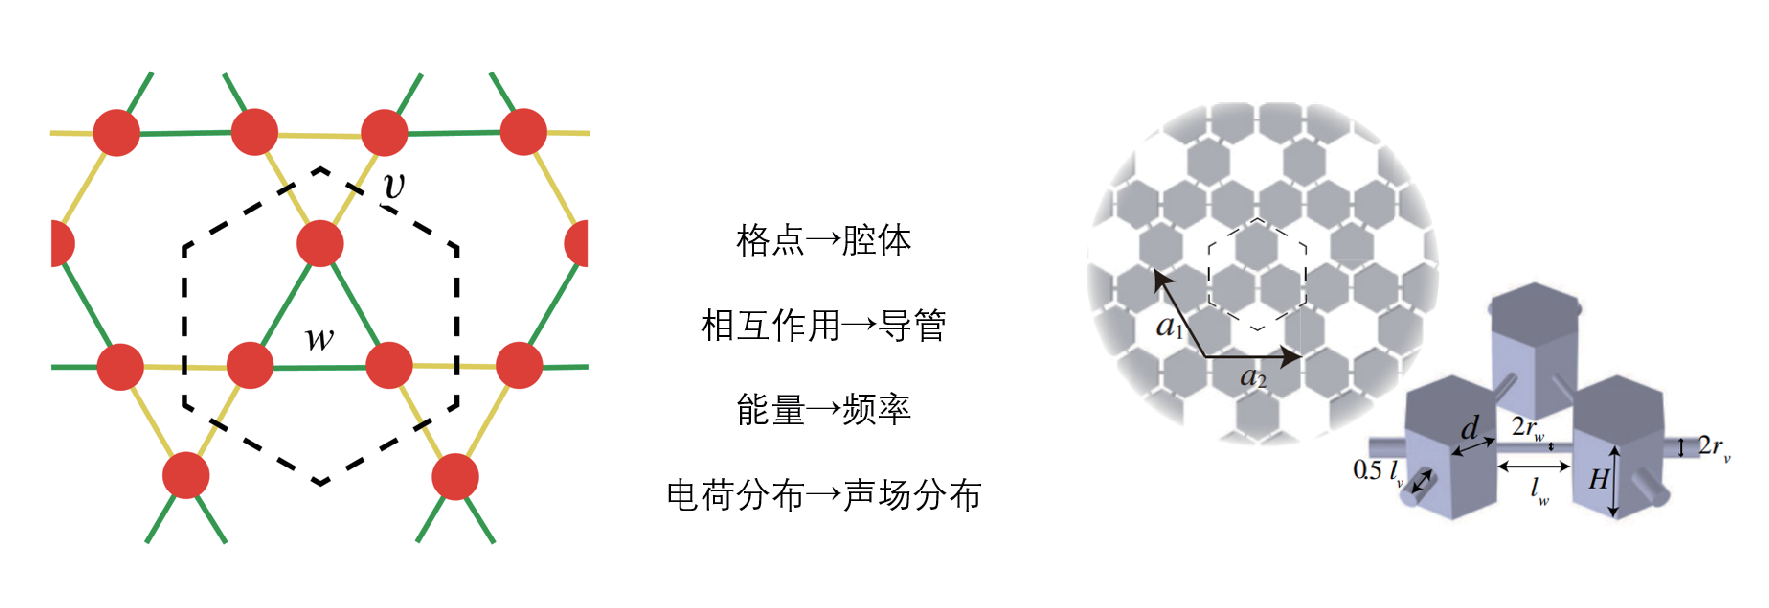
\includegraphics[width=1\textwidth]{images/fig3-1.eps} 
  \caption{以Kagome结构为例,电子系统与声学系统存在显著的相似性。}
  \label{fig_3_1}
\end{figure}

在物理学中,电子系统与声学系统存在显著的相似性。电子系统里,格点、相互作用、能量、电荷分布是关键要素;而在声学系统中,可类比为腔体、导管、频率、声场分布。以图\ref{fig_3_1}的Kagome晶格为例,以下是电子系统和声学系统中几个要素的相似性详细解释:
\begin{itemize}
  \item 格点与腔体:在电子系统的晶格模型中,格点是电子所处的位置,电子在这些格点上具有一定的能量状态和量子特性。格点的排列和相互关系决定了电子的能带结构等重要物理性质。而在声学系统中,我们可以把单个腔体看作是一个共振单元,它也具有共振频率和对应的共振模式。而使用周期排列的声学腔体,可以模仿电子晶格空间排列,构造相同的空间对称性。二者在离散化的单个单元共振和多个单元的空间排列上,存在一定的相似性。
  \item 电子系统的相互作用与声学导管:在电子系统的晶格模型中,电子在晶格中的跳跃等过程可以看作是一种相互作用,它决定了电子在不同格点之间的转移和能量传递。在声学系统中,我们可以在腔体之间连接导管,为不同腔体提供相互作用,并通过调节导管的参数实现对这种相互作用的大小和正负符号的调节。二者在单元和单元的相互作用上存在一定的相似性。
  \item 能量与频率:在电子系统中,薛定谔方程用于求解电子能量的本征值问题,其能量以离散本征值呈现,相应本征向量描述电子运动状态 。当处于周期结构时,电子会形成能带,其特性受晶格周期性影响。在声学系统里,波动方程的求解同样属于本征值问题,频率(或者频率的平方)作为本征向量,其离散取值决定声波传播模式。在周期结构的声学体系中,声波也会形成类似的能带结构,该结构与声学单元的周期性排列密切相关。二者在本征值问题架构及周期结构下形成能带的特性上,展现出显著的相似性。 
  \item 电荷分布与声场分布:在电子系统中,电荷分布反映了电子于空间的分布态势,它与电子的能量状态、相互作用及外部电场紧密相连,电荷分布的不均匀会引发电场等物理效应,对电子系统的电学性质和物理行为产生影响。在声学系统里,声场分布体现了声波在空间中的强度、相位分布状况,腔体和导管的结构以及声波传播特性致使声场在空间呈现不同分布模式。二者相似之处在于,它们均是描述各自系统内物理量在空间的分布,且这种分布都会显著影响系统与其他物质的相互作用,以及整个系统的性能表现。特别地,在拓扑绝缘体的研究中,我们可以观测二者的场分布,从而观测其拓扑性质。 
\end{itemize}

从类比的相似性出发,我们构造了如图\ref{fig_3_1}所示的声学结构。图中周期结构以C$_{3}$对称性排列,其中$a_1$和$a_2$是两个方向晶格基矢的大小,用于描述晶格的周期性结构。右侧展示了单个晶格的三维结构:一个由三个相同的六边形亥姆霍兹谐振器通过波导管连接而成的三角晶格,并考虑$C_3$对称性和平移不变性,即所有谐振器是相同的,其边长为$d$,高度为$H$。$l_w$和$l_v$分别对应胞内耦合的导管和胞间导管的长度,$r_w$和$r_v$是分别对应胞内耦合的导管和胞间导管的半径。从直觉上而言,当连接两个腔体的导管的长度更短,横截面积更大,此时两个腔体之间的相互作用更大,对应电子系统中更大的格点间的跳跃\cite{j4,h8}。

\section{Kagome晶格的声学哈密顿量}

\begin{figure}[h!]
  \centering
  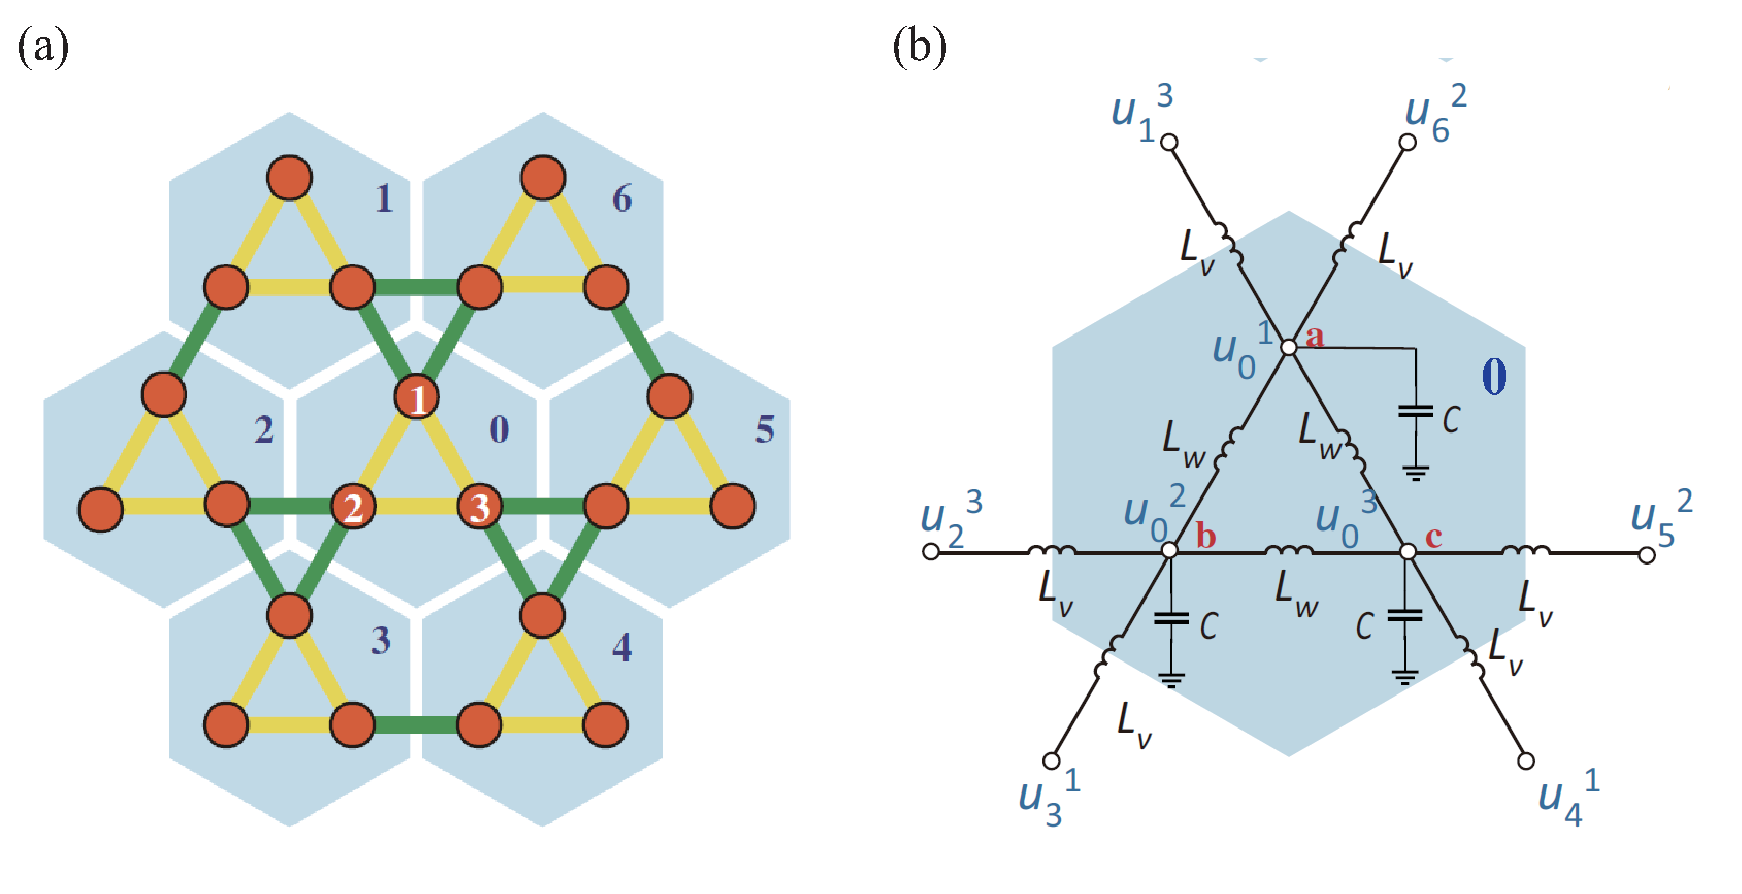
\includegraphics[width=1\textwidth]{images/fig3-2.eps} 
  \caption{Kagome声学系统体晶格的等效电路:
  (a)元胞Kagome晶格结构,其中晶格0居中,周围相邻的晶格分别编号为1到6。(b)晶格0的等效电路图。
  }
  \label{fig_3_2}
\end{figure}

如上一节所述,电子系统和声学系统有着相似性,我们可以构造声学腔管结构来类别电子Kagome晶格,也可以通过直觉调控其胞间和胞内的相互作用。在本节中,从声电类比方法出发,我们在亚波长尺度下从传统声学的角度严格推导出具有二维周期排列Kagome晶格的声共振系统的哈密顿量,从而揭示理论模型中的胞内或胞间跳跃与实际物理系统中的声学参数之间的联系。对于有限大结构,由于体,边,角上晶格的相邻晶格数量不同,我们也分别作了讨论。

首先,我们可以通过声学-电学类比来定义声学系统的 lumped 参数模型。如图\ref{fig_3_2}(a)所示,对于在周期结构中的晶格0而言,其周围有六个最近邻晶格,编号为1到6。单个晶格0的等效电路图如图\ref{fig_3_2}所示。在该电路模型中,腔体被表示为电容 \( C \),波导被表示为电感 \( L_v \) 和 \( L_w \)。具体公式如下:
\begin{equation} \label{eq3-1}
  C = \frac{V}{\rho c^2},
\end{equation}
\begin{equation} \label{eq3-2}
  L_v = \frac{\rho (l_v + 1.7r_v)}{\pi r_v^2}, \quad L_w = \frac{\rho (l_w + 1.7r_w)}{\pi r_w^2},
\end{equation}
其中,\( V \) 是腔体的体积,\( \rho \) 是空气的密度,\( c \) 是声速,\( r_v \) 和 \( r_w \) 分别是波导的半径,\( l_v \) 和 \( l_w \) 是它们的长度。

通过应用基尔霍夫电流定律,我们可以得到了描述声学波动的方程。对于周期性结构,腔体的声压在每个晶格点处满足如下方程:
\begin{subequations}\label{eq3-3}
  \begin{align}
  -(2w + 2v)u_{1}^{0} + wu_{2}^{0} + wu_{3}^{0} + vu_{2}^{6} + vu_{3}^{1} &= \omega^{2}u_{1}^{0}\label{eq:sub1}\\
  -(2w + 2v)u_{2}^{0} + wu_{3}^{0} + wu_{1}^{0} + vu_{3}^{2} + vu_{1}^{3} &= \omega^{2}u_{2}^{0}\label{eq:sub2}\\
  -(2w + 2v)u_{3}^{0} + wu_{1}^{0} + wu_{2}^{0} + vu_{1}^{4} + vu_{2}^{5} &= \omega^{2}u_{3}^{0}\label{eq:sub3}
  \end{align}
\end{subequations}
其中,$u_m^n$表示第$m$个晶格的第$n$个空腔中的声压,且$v = -1/L_vC$,$w = -1/L_wC$。对于一个周期性结构,它保证了$u_m^n$可以被描述为布洛赫波函数,方程(3)可以重写为矢量形式:
\begin{equation}\label{eq3-4}
  \mathcal{H}_{0}\mathbf{u} = \omega^{2}\mathbf{u},
\end{equation}
其中,$\mathbf{u} = [u_0^1\ u_0^2\ u_0^3]^{\mathrm{T}}$,并且$\mathcal{H}_{0}$可以表示为:
\begin{equation}\label{eq3-5}
  \mathcal{H}_{0}(\mathbf{k}) = 
  \begin{bmatrix}
  -2w - 2v & w + ve^{j\mathbf{k}\cdot(\mathbf{a}_{1}+\mathbf{a}_{2})} & w + ve^{j\mathbf{k}\cdot\mathbf{a}_{1}} \\
  w + ve^{-j\mathbf{k}\cdot(\mathbf{a}_{1}+\mathbf{a}_{2})} & -2w - 2v & w + ve^{-j\mathbf{k}\cdot\mathbf{a}_{2}} \\
  w + ve^{-j\mathbf{k}\cdot\mathbf{a}_{1}} & w + ve^{j\mathbf{k}\cdot\mathbf{a}_{2}} & -2w - 2v
  \end{bmatrix}
\end{equation}
其中,$\mathbf{k}$是布洛赫波矢,$\mathbf{a}_{1}$、$\mathbf{a}_{2}$表示晶格常数。显然可以看出,求解周期结构的共振频率及其相应的特征模式可归结于求解$\mathcal{H}_{0}$的本征值问题,这与电子系统的哈密顿量相对应,$w$和$v$对应于Kagome晶格的胞内跳跃和胞间跳跃。我们把$\mathcal{H}_{0}$称为无限大周期排列的Kagome结构的声学哈密顿量。

\begin{figure}[h!]
  \centering
  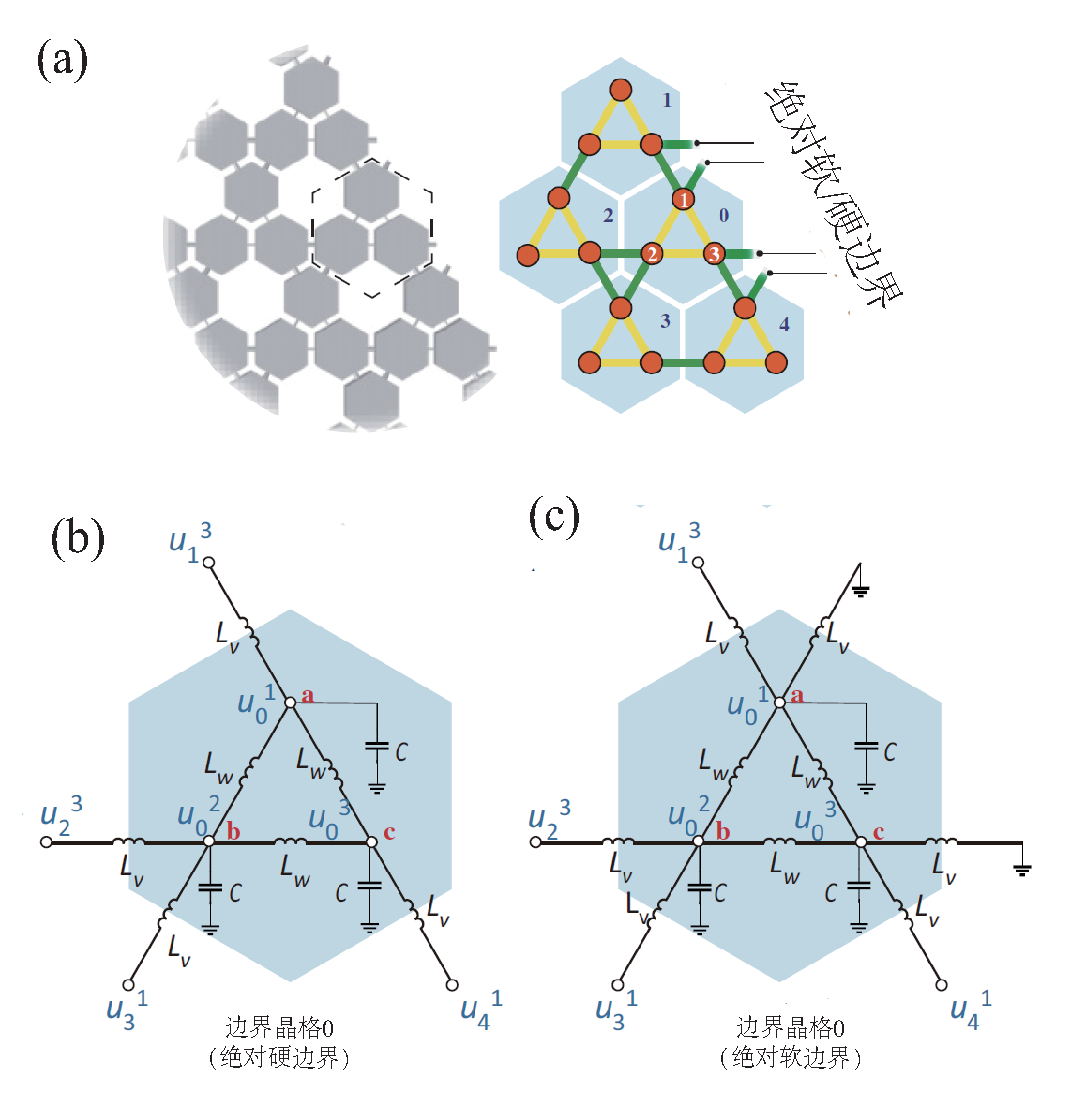
\includegraphics[width=1\textwidth]{images/fig3-3.eps} 
  \caption{Kagome声学系统边界上晶格的等效电路:
  (a)边界上Kagome晶格结构,其中晶格0为边上晶格,周围相邻的晶格分别编号为1到4。(b)绝对硬边界时晶格0的等效电路图。(b)绝对软边界时晶格0的等效电路图。
  }
  \label{fig_3_3}
\end{figure}

我们注意到,对于周期系统,该结构相应哈密顿量的对角项(式\ref{eq3-5})是相同的。然而,若考虑有限大系统的边界,由于边、角晶格相邻晶格的数目体晶格相邻晶格数目不同,这会导致哈密顿量的对角项。有限结构哈密顿量中对角项的差异会对拓扑性质产生巨大影响,这是由于广义手征对称性的差异所致,而广义手征对称性保护着拓扑态。我们以边界晶格为例说明这种有限大系统边界上哈密顿量随边界条件的改变,如图\ref{fig_3_3}所示,我们假设在有限结构的边缘存在一个晶格0。与图\ref{fig_3_2}(a)相比,图\ref{fig_3_3}(a)中的相邻晶格5和6被与之相连的最外层管道的硬边界或软边界所取代。在集总电路模型中,硬边界相当于断路情况,而软边界相当于接地,分别如图\ref{fig_3_3}(b)和图\ref{fig_3_3}(c)所示。相应地,对于硬边界情况,边缘晶格的方程可如下获得:
\begin{subequations}\label{eq3-6}
  \begin{align}
  -(2w + v)u_{0}^{1} + wu_{0}^{2} + wu_{0}^{3} + vu_{1}^{3} &= \omega^{2}u_{0}^{1}, \\
  -(2w + 2v)u_{0}^{2} + wu_{0}^{3} + wu_{0}^{1} + vu_{2}^{3} + vu_{3}^{1} &= \omega^{2}u_{0}^{2}, \\
  -(2w + v)u_{0}^{3} + wu_{0}^{1} + wu_{0}^{2} + vu_{4}^{1} &= \omega^{2}u_{0}^{3}, \
  \end{align}
\end{subequations}
而软边界情况的公式为:
\begin{subequations}\label{eq3-7}
  \begin{align}
  -(2w + 2v)u_{0}^{1} + wu_{0}^{2} + wu_{0}^{3} + vu_{1}^{3} &= \omega^{2}u_{0}^{1}, \\
  -(2w + 2v)u_{0}^{2} + wu_{0}^{3} + wu_{0}^{1} + vu_{2}^{3} + vu_{3}^{1} &= \omega^{2}u_{0}^{2}, \\
  -(2w + 2v)u_{0}^{3} + wu_{0}^{1} + wu_{0}^{2} + vu_{4}^{1} &= \omega^{2}u_{0}^{3}. 
  \end{align}
\end{subequations}
将方程\ref{eq3-6}与方程\ref{eq3-7}进行比较,可以明显看出边界条件的影响恰好反映在哈密顿量对角项的差异上。总体而言,软边界使得所有晶格(包括体晶格和边界晶格)的对角项都等于$-(2w + 2v)$。从这个角度来看,应用绝对软边界的有限大声学系统可以被视为是更接近电子系统的类比。

\section{无限大周期排列的Kagome晶格的拓扑相变}

\begin{figure}[h!]
  \centering
  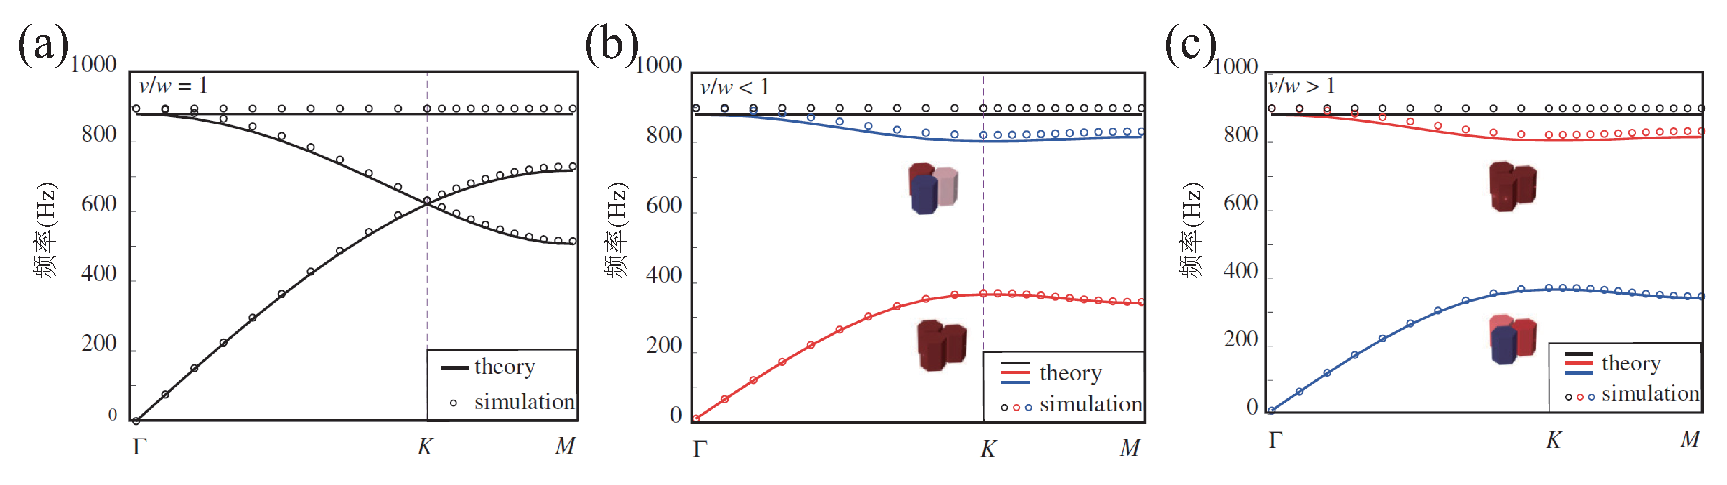
\includegraphics[width=1\textwidth]{images/fig3-4.eps} 
  \caption{Kagome声学系统的体能带:
  (a)$w=v$时能带结构,直线表示理论计算结果,圆点表示有限元仿真结果。(b)$w>v$时能带结构,直线表示理论计算结果,圆点表示有限元仿真结果。(c)$w<v$时能带结构,直线表示理论计算结果,圆点表示有限元仿真结果。
  }
  \label{fig_3_4}
\end{figure}

上一节中,我们推导了这种腔管结构的声学方程。接下来,我们研究这种晶格周期排列时的拓扑性质。在图\ref{fig_3_4}中,谐振器的边长和高度分别为$d = 10$(mm)和$h = 25$(mm)。波导管的长度为$l_w = l_v = 2.5$(mm),$V$是腔体的体积。空气的质量密度和相应的声速分别定义为$\rho = 1.23$(kg/m³)和$c = 343$(m/s)。一般来说,带反转发生在胞间跳跃的变化处,此模型中的胞间跳跃和胞内跳跃由胞间管半径$r_w$和胞内管半径$r_v$分别确定。

使用COMSOL Multiphysics进行模拟,图\ref{fig_3_4}描绘了当$r_w = r_v = 0.55$(mm),$r_w = 0.75$(mm)且$r_v = 0.3$(mm),$r_v = 0.3$(mm)且$r_v = 0.75$(mm)时的能带结构。由$v = -1/L_vC$,$w = -1/L_wC$,这三种情况分别对应$v/w=1$,$v/w<1$和$v/w>1$。其中,直线是我们使用上一节的方法计算的能带图,而圆点是有限元仿真结果。可以看到二者基本相吻合。三个图中的平带来自于相消干涉,这导致了紧致局域态,而另外两条能带反映了拓扑性质\cite{C3-1,C3-2}。可以明显看出,当$r_w = r_v$时,存在一个受对称性保护的狄拉克锥,这表明拓扑相变的临界点。通过观察(b)图和(c)图狄拉克锥打开又闭合时,两条能带的对应的声场分布(图中的插图部分),我们可以观察到了能带反转现象。对于$C_3$对称晶格,体极化$p_l$定义为:
\begin{equation} \label{eq3-8}
  e^{-i\pi p_l} = \prod_{n \in \text{occ}} \frac{\theta_n(\mathbf{K})}{\theta_n(\Gamma)},
\end{equation}
其中$\theta_n(\mathbf{k}) = (u_n(\mathbf{k})|R_{3}|u_n(\mathbf{k}))$是通过将三重对称算子$R_3$(旋转$2\pi/3$)应用于晶格高对称点处相应的布洛赫波函数$u_n(\mathbf{k})$计算得到的,“occ”表示占据带。

由于通过电声类比推导出的声学系统中的哈密顿量与参考文献\cite{f6}中凝聚态物理的情况相同,所以为了获得以体极化表征的拓扑不变量,我们可以使用Wilson Loop方法来计算Wannier center,描述如下\cite{i5}:
\[W_{k_1,k_2 + 2\pi \leftarrow k_2}|\nu_{\mathbf{k}}^j\rangle = e^{i2\pi \nu_2}|\nu_{\mathbf{k}}^j\rangle,\quad (A1)\]
其中Wilson Loop定义为:
\begin{equation}\label{eq3-9}
  \begin{aligned}
  W_{k_1,k_2 + 2\pi \leftarrow k_2} &= \langle u_{k_1,k_2 + N\delta k}|u_{k_1,k_2 + (N - 1)\delta k}\rangle\\
  &\times \langle u_{k_1,k_2 + (N - 1)\delta k}|u_{k_1,k_2 + (N - 2)\delta k}\rangle \cdots\\
  &\times \langle u_{k_1,k_2 + 2\delta k}|u_{k_1,k_2 + \delta k}\rangle\langle u_{k_1,k_2 + \delta k}|u_{k_1,k_2}\rangle
  \end{aligned}
\end{equation}
在方程\ref{eq3-9}中,\(\nu\)是Wannier center,\(j\)表示占据的能带。\(N\)和\(\delta k\)表示\(k_2\)方向上的离散化。接下来,可以得到体极化:
\begin{equation} \label{eq3-10}
  p_1 = \frac{1}{N} \sum_{j,k_1} \nu_2^j(k_1),
\end{equation}

\begin{figure}[h!]
  \centering
  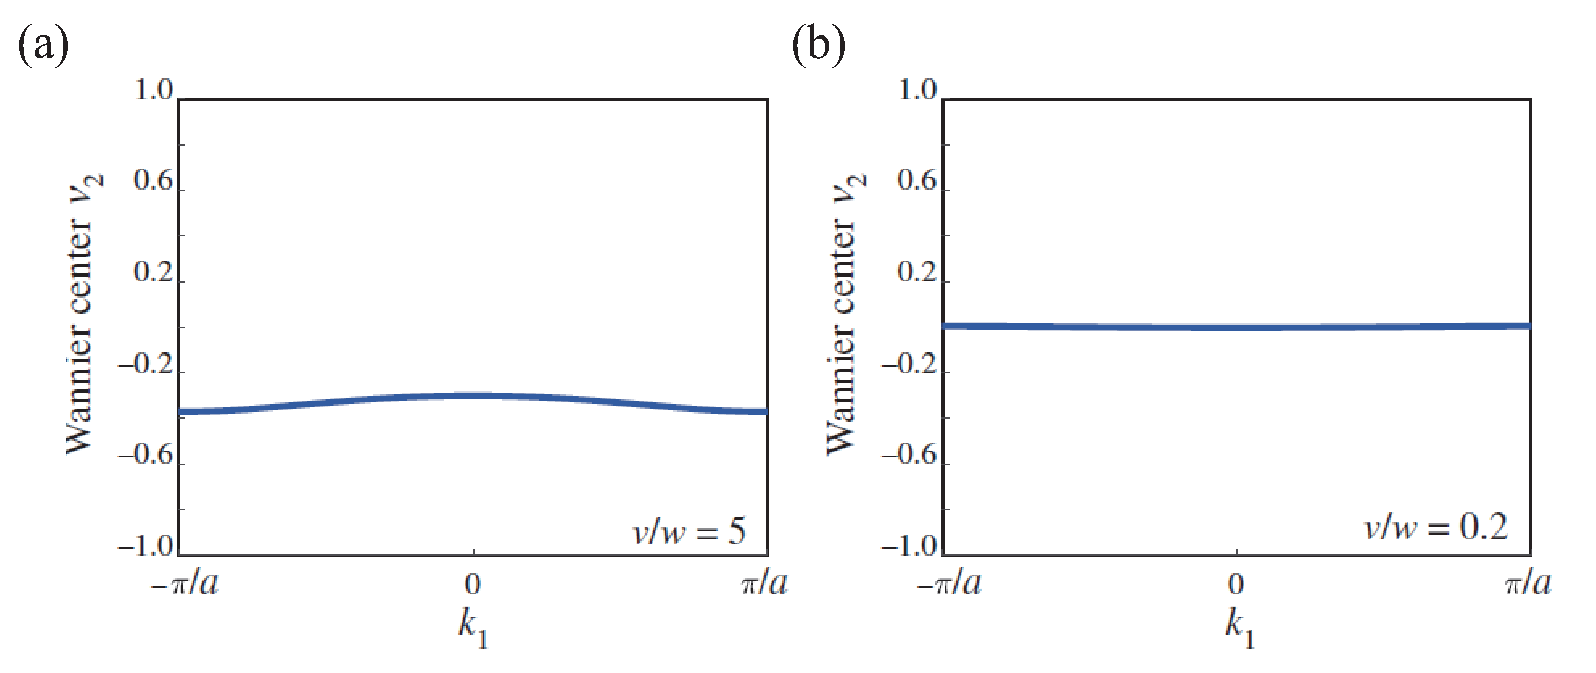
\includegraphics[width=1\textwidth]{images/fig3-5.eps} 
  \caption{当(a)\(v/w = 5\)和(b)\(v/w = 0.2\)时Kagome晶格的Wannier能带。
  }
  \label{fig_3_5}
\end{figure}

在图\ref{fig_3_5}中,我们展示了当\(v/w = 5\)和\(v/w = 0.2\)时万尼尔中心的数值结果。根据方程\ref{eq3-10},\(v/w = 5\)时的体极化是\(-1/3\),而\(v/w = 0.2\)时的体极化是\(0\),这表明前者情况在拓扑上是非平庸的,而后者情况在拓扑上是平庸的。因此体极化可表示为:
\begin{equation} \label{eq3-11}
  (p_1,p_2) = 
  \begin{cases}
  (-1/3,-1/3), & w < v \\
  (0,0), & w > v
  \end{cases}
\end{equation}
因此,当$w < v$时的非零极化表明了能带的非平庸拓扑相,而当$w > v$时则表示平庸相。由于所有原子被认为是相同的,边界诱导的填充异常预计将沿着非平庸体极化情况被诱导,这由拓扑边界态的存在表示,此时边界是开放的。同时,当所有原子在热力学极限下相同时,也可以诱导出由低维拓扑角态表征的角诱导填充异常\cite{C3-3}。

到目前为止,我们讨论的是所有原子在热力学极限下相同的情况。然而,在下一节中,我们将展示当涉及到封闭经典系统时,系统的onsite能量(体现为哈密顿量的对角项)总是受到边界的影响。

\section{有限大带状排列的Kagome晶格的拓扑态}

\begin{figure}[h!]
  \centering
  \includegraphics[width=1\textwidth]{images/fig3-6.eps} 
  \caption{带状Kagome声学晶格的能带:
  (a) 带状超晶格的示意图。该带状结构沿$x$方向延伸,并在$y$方向上由硬边界或软边界(用蓝色线标记)包围。(b) $k = 0$时边界态的声压场分布。(c) 具有硬边界的超晶格的能带结构。(d) 具有软边界的超晶格的能带结构。
  }
  \label{fig_3_6}
\end{figure}

\begin{figure}[h!]
  \centering
  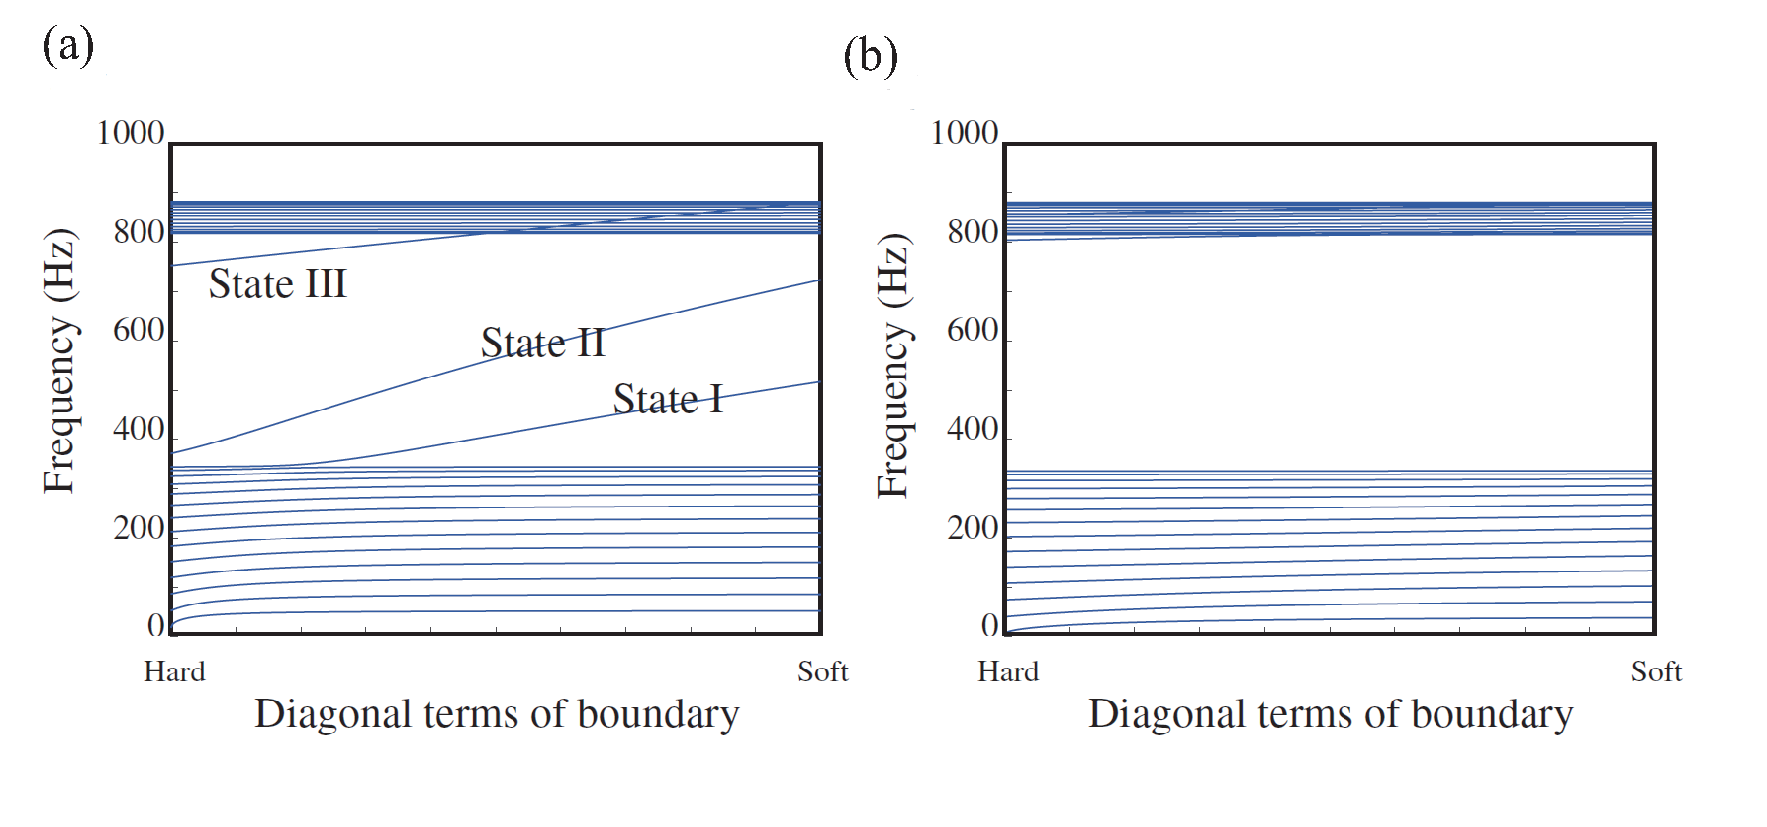
\includegraphics[width=1\textwidth]{images/fig3-7.eps} 
  \caption{当(a)\(v/w = 5\)和(b)\(v/w = 0.2\)时,随着边界对角项的变化(即从绝对硬边界过渡到绝对软边界),能带结构的变化。}
  \label{fig_3_7}
\end{figure}

\begin{figure}[h!]
  \centering
  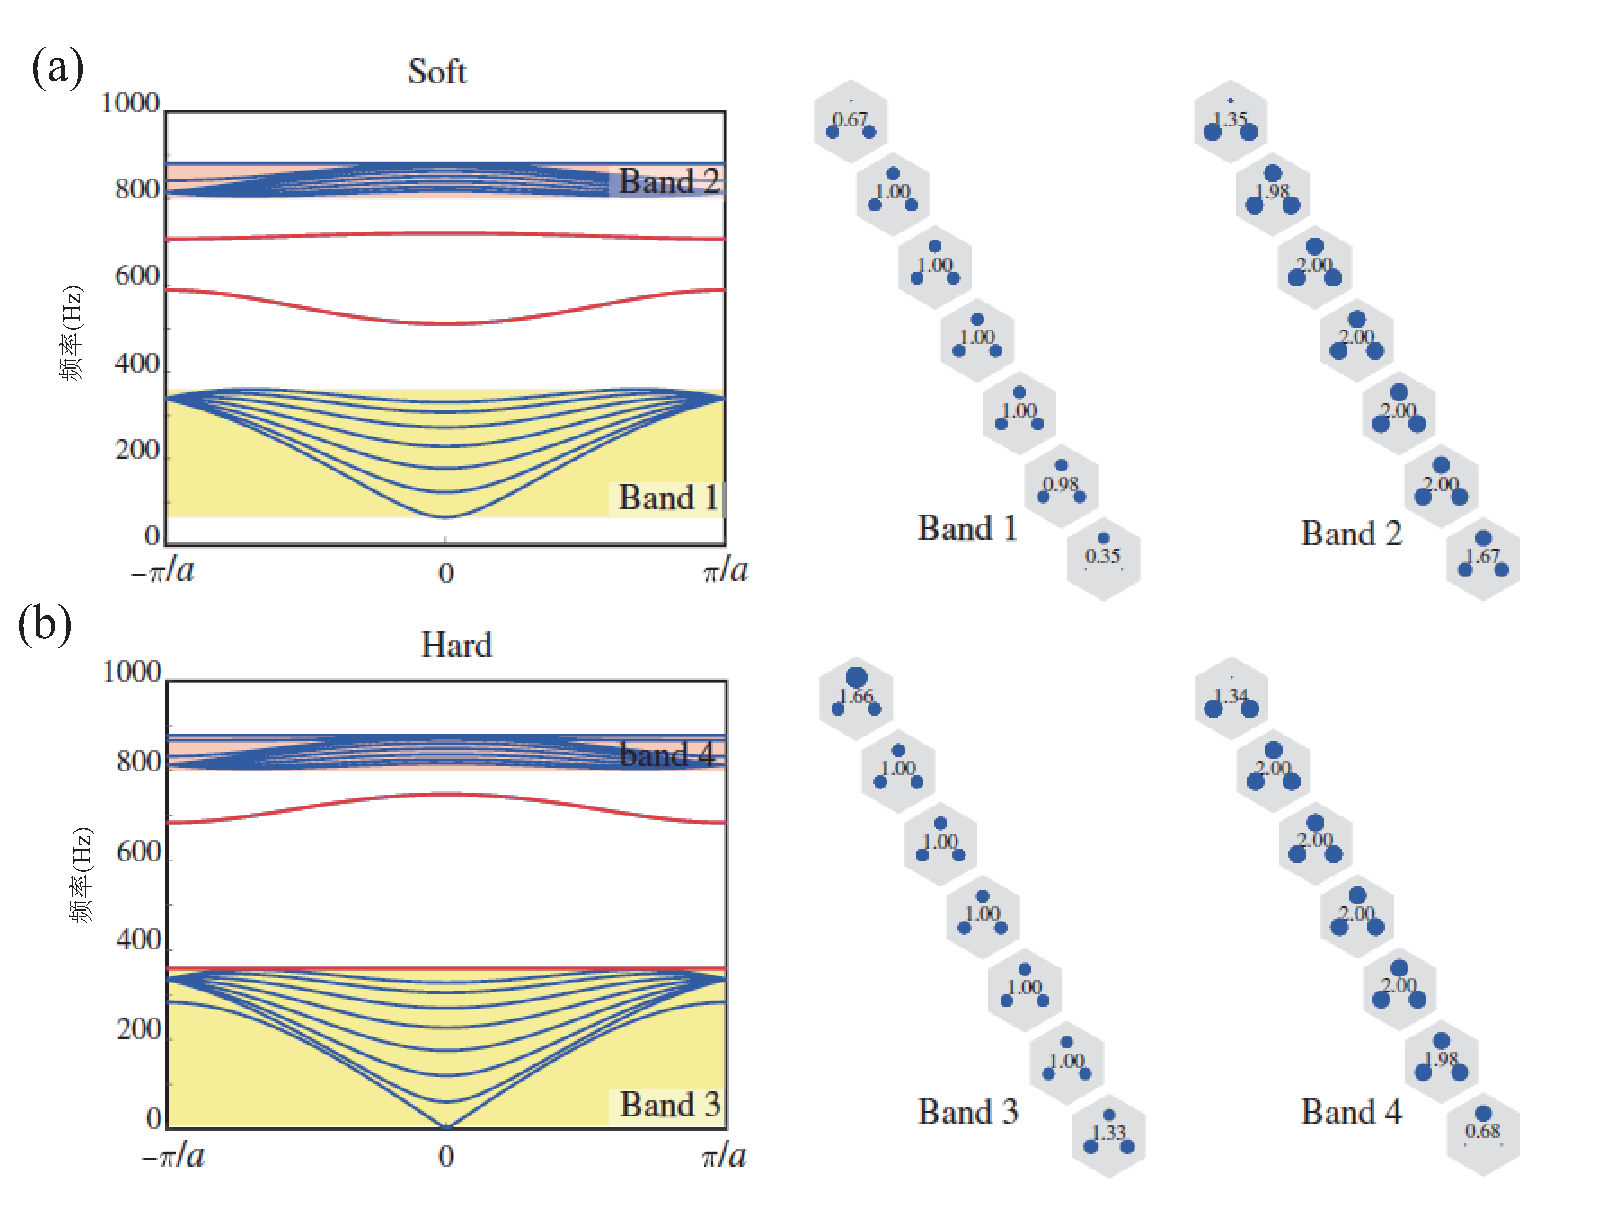
\includegraphics[width=1\textwidth]{images/fig3-8.eps} 
  \caption{当\(v/w = 5\)时,具有(a)绝对软边界和(b)硬边界的带状结构的局域态密度。}
  \label{fig_3_8}
\end{figure}

\begin{figure}[h!]
  \centering
  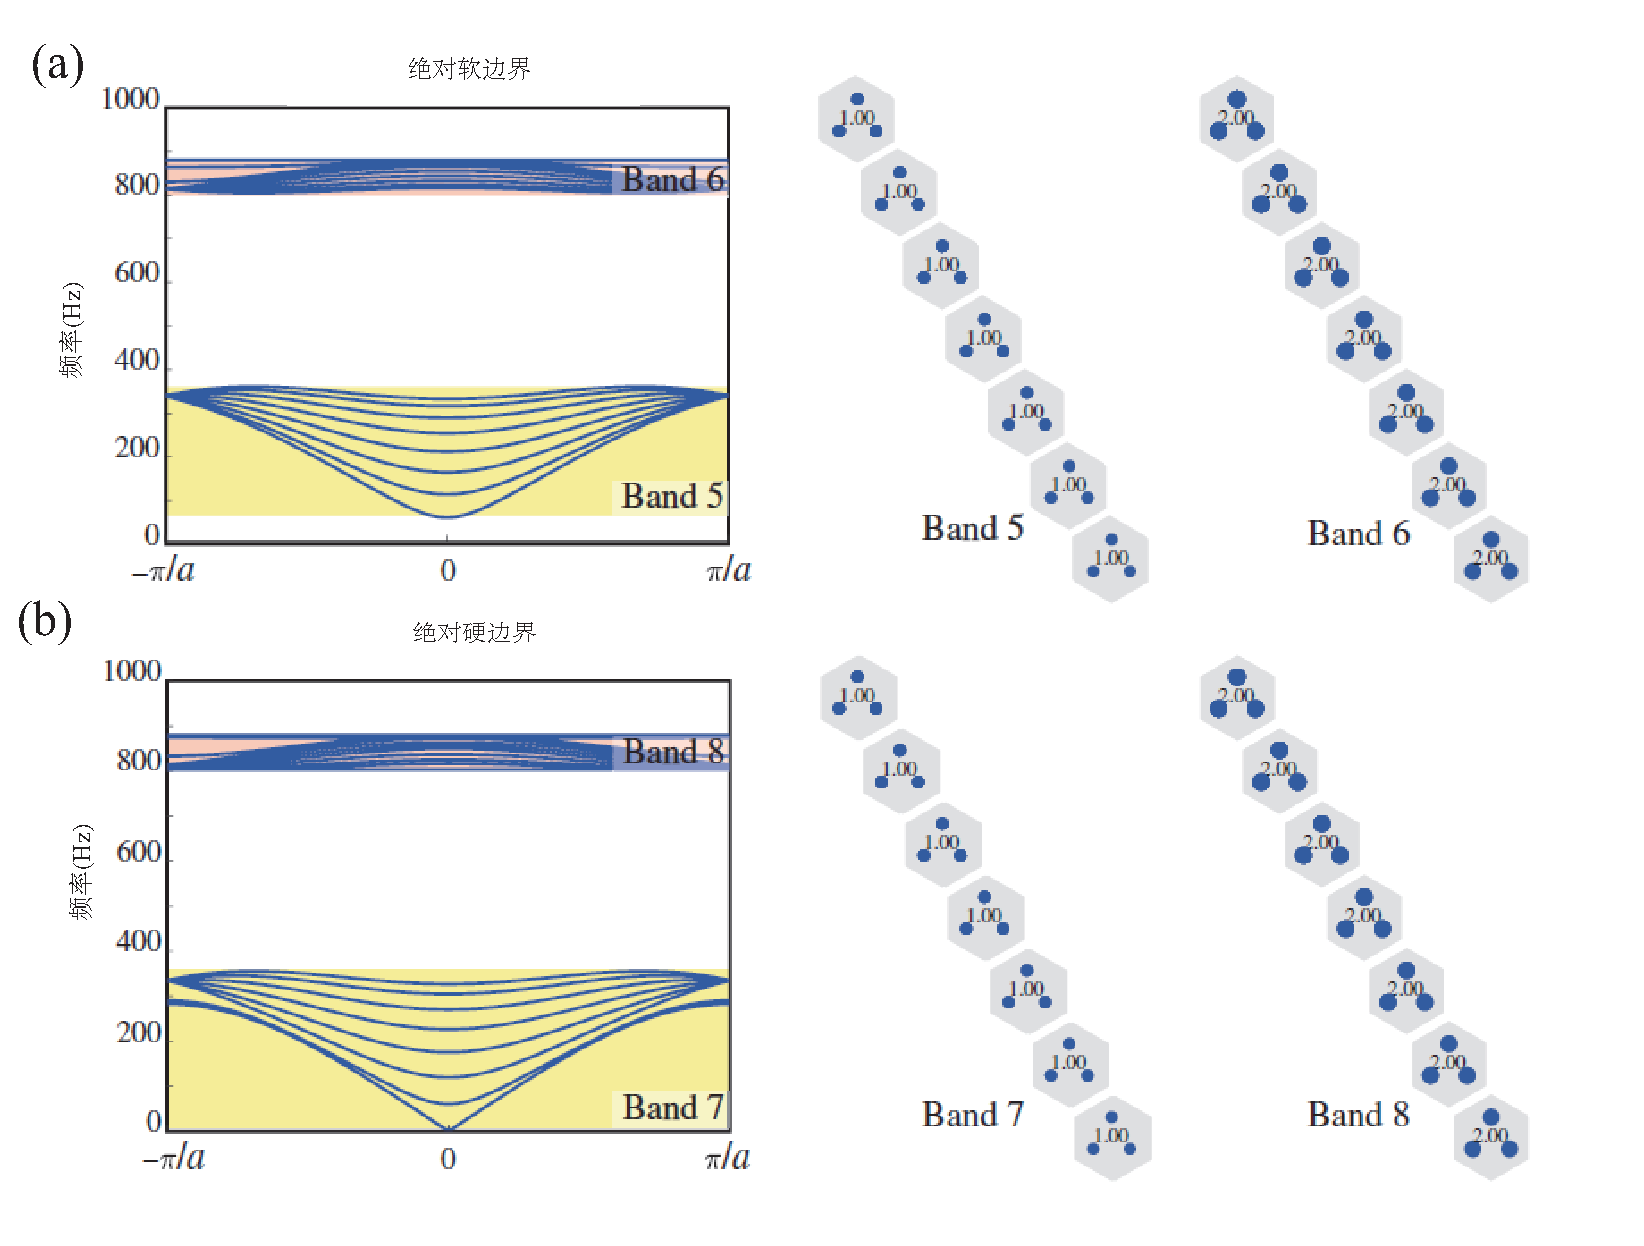
\includegraphics[width=1\textwidth]{images/fig3-9.eps} 
  \caption{当\(v/w = 0.2\)时,具有(a)绝对软边界和(b)硬边界的带状结构的局域态密度。}
  \label{fig_3_9}
\end{figure}

\begin{figure}[h!]
  \centering
  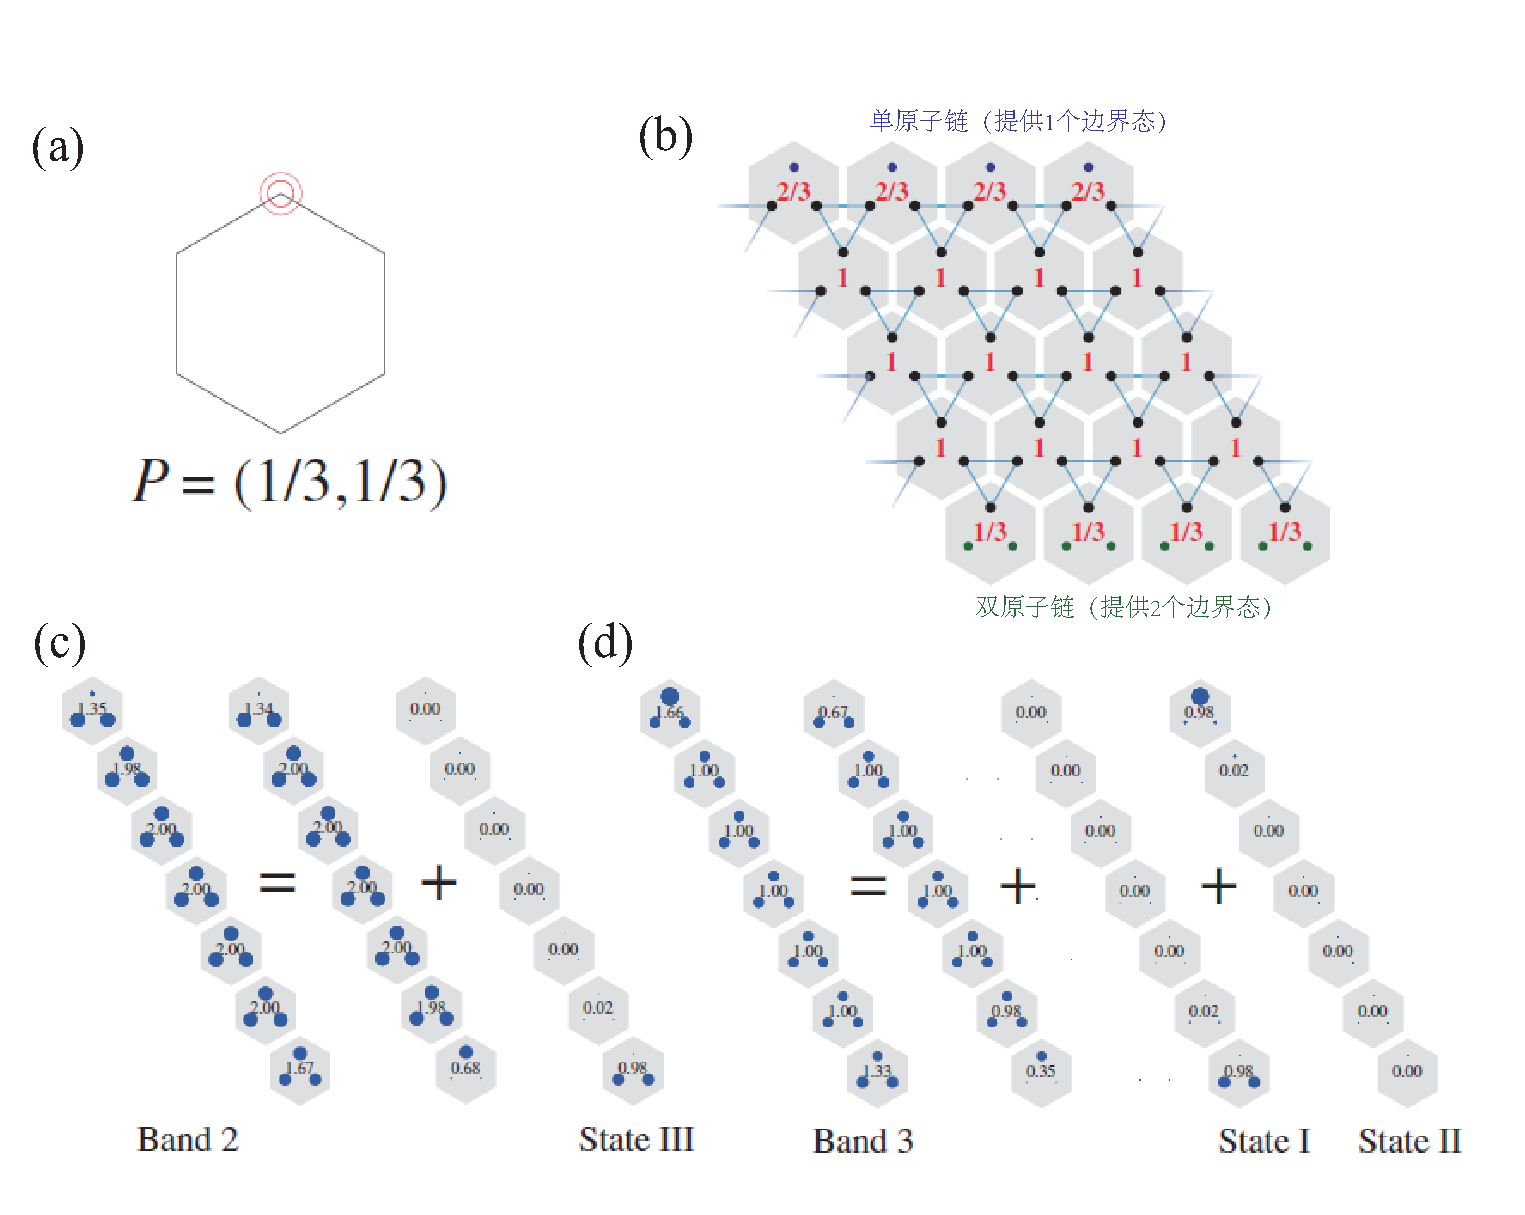
\includegraphics[width=1\textwidth]{images/fig3-10.eps} 
  \caption{(a)具有\(C_3\)对称性且\(\mathbf{P}=(-1/3,-1/3)\)的Wyckoff位置。(b)Kagome带状结构的体电荷和边缘电荷。(c)Band 2中的束缚态。(d)Band 3中的束缚态。}
  \label{fig_3_10}
\end{figure}

在上一节里,我们研究了无限大周期结构的Kagome晶格的能带结构和拓扑相变。在本节中,我们讨论半无限情形。如图3(a)所示,由八个非平庸的Kagome晶格组成的带状超晶格,其中$v/w = 5$,结构在y方向是有限的,在x方向是周期性的。值得注意的是,由于$C_3$对称性,上边缘和下边缘的几何形状是不同的\cite{C3-4}。关键的是,本工作中不是通过缺乏非平庸域与所谓的平庸“环境”之间的相互作用界面来实现,而是仅通过硬边界或软边界将上边缘和下边缘连接起来,从而使用边界条件限制了y方向。图\ref{fig_3_6}(c)和3(d)分别描绘了具有硬边界和软边界的超晶格的能带结构,其相应的拓扑模式在图\ref{fig_3_6}(b)中呈现。可以看出,在本征频率中这些模式是多样的,并且在不同情况下模式是不同的。对于硬边界情况,较低频率的模式位于上边界,但软边界情况则相反。尽管硬边界和软边界这两种拓扑状态仅出现在非平庸结构中且在平庸结构中消失,但从它们的模式来看,它们可能有不同的起源。因此,通过应用不同的边界条件,拓扑状态的存在是不同的。这种差异性可以使用态的局域密度\cite{C3-5}来解释。

接下来,我们来详细解释带状结构中软边界和硬边界的带隙内模式的差异性。实际上,在非平庸结构中有三个拓扑边界态,但它们并非都是带隙内态。这三个拓扑态的频率随不同边界条件而变化,这导致了软边界和硬边界的带隙内模式的差异。为了证实这些,我们将对角项从$-v$(硬边界)设置为 0(软边界),并研究$ k = 0 $时的能带结构。在非平庸晶格中,出现了标记为State I、State II和State III的三个拓扑态(如图\ref{fig_3_7}(a)所示)。对于绝对软边界,这三个拓扑态中的上态埋在体带中。对于绝对硬边界,上态下降到带隙中,而中间态下降到下体带的边缘,下态埋在下体带中。在平庸情况(图\ref{fig_3_7}(b))中,所有三个拓扑边界态都消失。此外,我们计算了非平庸结构和平庸结构中两种边界条件的局域态密度(LDOS)\cite{C3-5},如图\ref{fig_3_8}和图\ref{fig_3_9}所示。在图\ref{fig_3_8}中,我们清楚地看到在非平庸结构中有边界态,而在图\ref{fig_3_9}中体和边界单元的模式密度几乎相等,表明它是拓扑平庸的,并且没有共振态或拓扑态。考虑图\ref{fig_3_10}(a)中所示的 Wyckoff 位置的 Wannier 轨道,其中 P = (-1/3, -1/3),Wyckoff 位置的 Wannier 中心和模式密度的分数部分在图\ref{fig_3_10}(b)中展示。此外,将图\ref{fig_3_8}中Band 2 和Band 3 的 LDOS 与图\ref{fig_3_10}(b)进行比较,我们可以找到连续体中的束缚态,如图\ref{fig_3_10}(c)和(d)所示。而且,图中的三个态都是拓扑保护模式。如图\ref{fig_3_10}(b)所示,上边缘充当单个原子,从而产生State I,而下边缘充当二聚化的双原子链,产生State II 和State III。

\section{有限大三角排列的Kagome晶格的拓扑态}

\begin{figure}[h!]
  \centering
  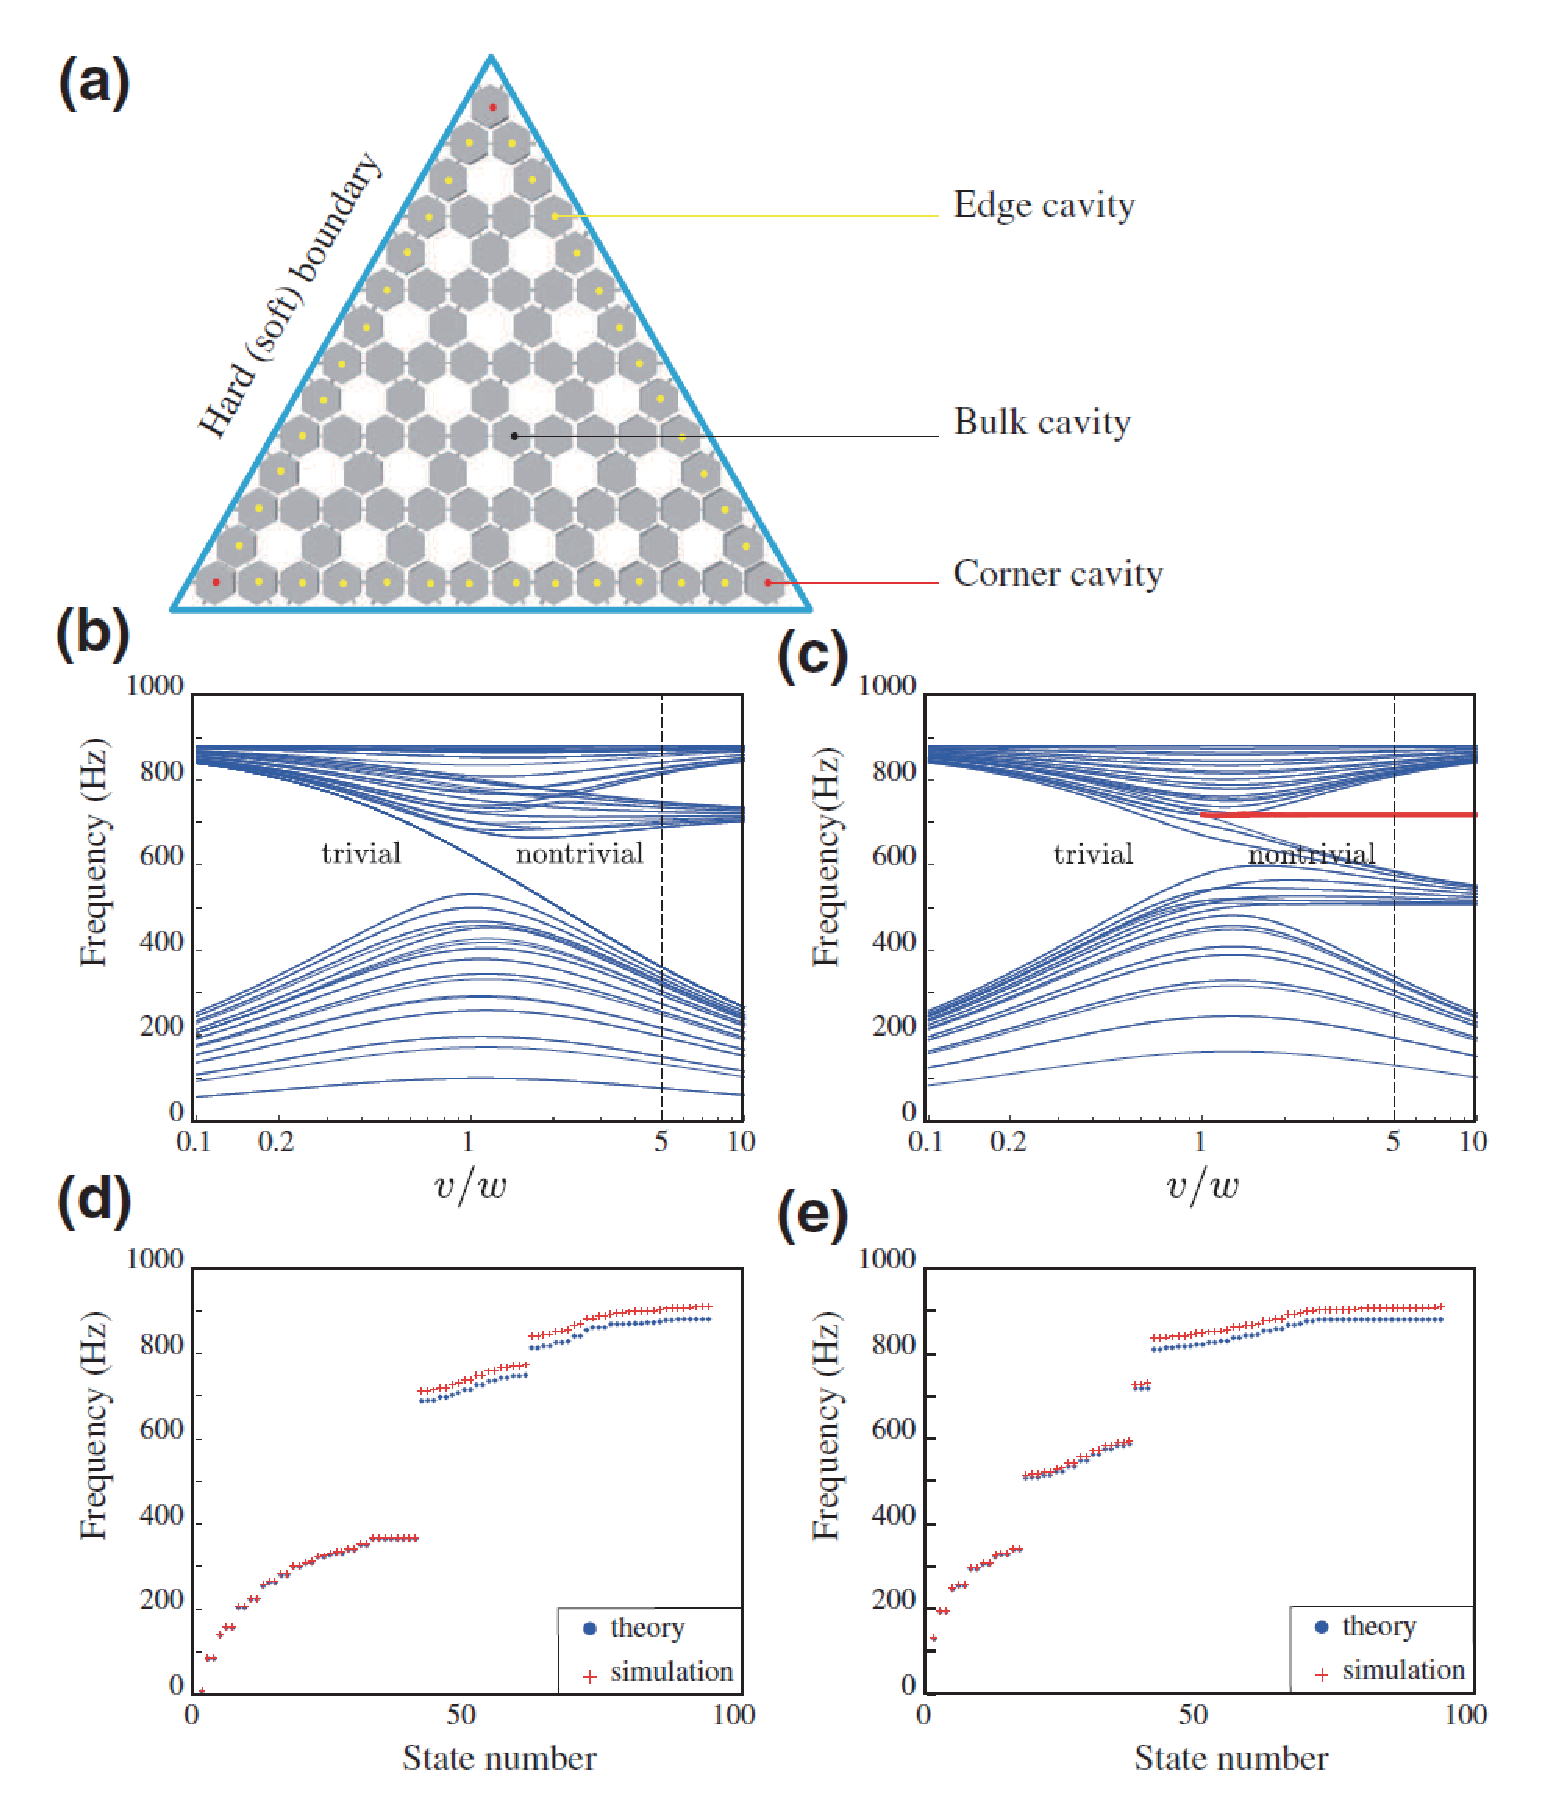
\includegraphics[width=1\textwidth]{images/fig3-11.eps} 
  \caption{(a) 带状超晶格的示意图。该带状结构沿x方向延伸,并在y方向上由硬边界或软边界(用蓝线标记)包围。(b) 在k = 0时边界态的声压场分布。(c) 具有硬边界的超晶格的能带结构。(d) 具有软边界的超晶格的能带结构。}
  \label{fig_3_11}
\end{figure}


此外,考虑到最外层边界条件,我们证明了在具有完全开放边界的二维材料中存在二阶拓扑态。图\ref{fig_3_11}(a)展示了由28个Kagome晶格组成的非平凡三角形结构,整个结构由硬(软)边界包围。因此,该结构中的晶格可以分别定义为体晶格、边缘晶格和角晶格。对于体晶格,有六个最近邻晶格,而边缘晶格有四个最近邻晶格,角晶格只有两个最近邻晶格。哈密顿量的对角项与边界条件之间的关系可以通过如表I所示的声电类比得到。

结果表明,具有软边界的哈密顿量中的所有对角项是等效的,而硬边界的对角项是不同的,这与第三节中的讨论相符。关键的是,图\ref{fig_3_11}(b)和(c)展示了在不同边界条件下能带结构随\(v/w\)比值的变化过程。结果中突出的是,只有在软边界条件下角态才能存在,这是由于与硬边界条件相比,\(C_3\)对称性和广义手性对称性的保持。此外,由于等效的在位项,在软边界条件下得到的哈密顿量\(\mathcal{H}_0\)严格对应于凝聚态物理中提出的拓扑绝缘体的理论模型。因此,诱导的角态(在图\ref{fig_3_11}(c)中用红线标记)恰好对应于零能态。我们通过以下方程计算角态的频率:
\begin{equation}\label{eq3-12}
  \begin{aligned}
  f_{corner} &= \frac{\sqrt{-2w - 2v}}{2\pi}\\
  &= \frac{1}{2\pi}\sqrt{\frac{2\pi c^2}{V}\left(\frac{r_v^2}{l_v + 1.7r_v}+\frac{r_w^2}{l_w + 1.7r_w}\right)}
  \end{aligned}
  \end{equation}
这里,我们设置\(v/w = 5\)来展示我们的结果。为了进行比较,理论结果和模拟结果分别如图\ref{fig_3_11}(d)和(e)所示。在我们使用方程\ref{eq3-12}的计算中,软边界条件下角态的频率为718Hz,模拟结果为727Hz。同时,边缘态和“零能”角态的理论和数值结果分别如图\ref{fig_3_12}(a)和(b)所示。

方程\ref{eq3-12}表明角态的频率仅与\(w\)和\(v\)有关。实际上,晶胞内跳跃\(w\)和晶胞间跳跃\(v\)完全决定了能带结构的形状,而对角项(换句话说,在位能)决定了频率的位置。在这种情况下,能带隙出现在\([\sqrt{-3w}/2\pi,\sqrt{-3v}/2\pi]\),这是从方程\ref{eq3-4}得到的,并且角态的频率可从方程\ref{eq3-12}得知。到目前为止,关于能带结构的所有具体信息都已知。这为我们应用高阶拓扑绝缘体以满足实际需求提供了方向。例如,当我们需要在特定频率下获得角态时,我们首先从方程\ref{eq3-12}确定晶胞内跳跃\(w\)和晶胞间跳跃\(v\)。然后,根据\(w = -1/L_wC\)和\(v = -1/L_vC\)的表达式,我们选择声学组件的适当阻抗值。最后,我们可以基于这些来设计腔体和管道的实际尺寸以满足实际尺寸需求。此外,该方法可以扩展到其他结构,如方形晶格或蜂窝晶格。

\begin{figure}[h!]
  \centering
  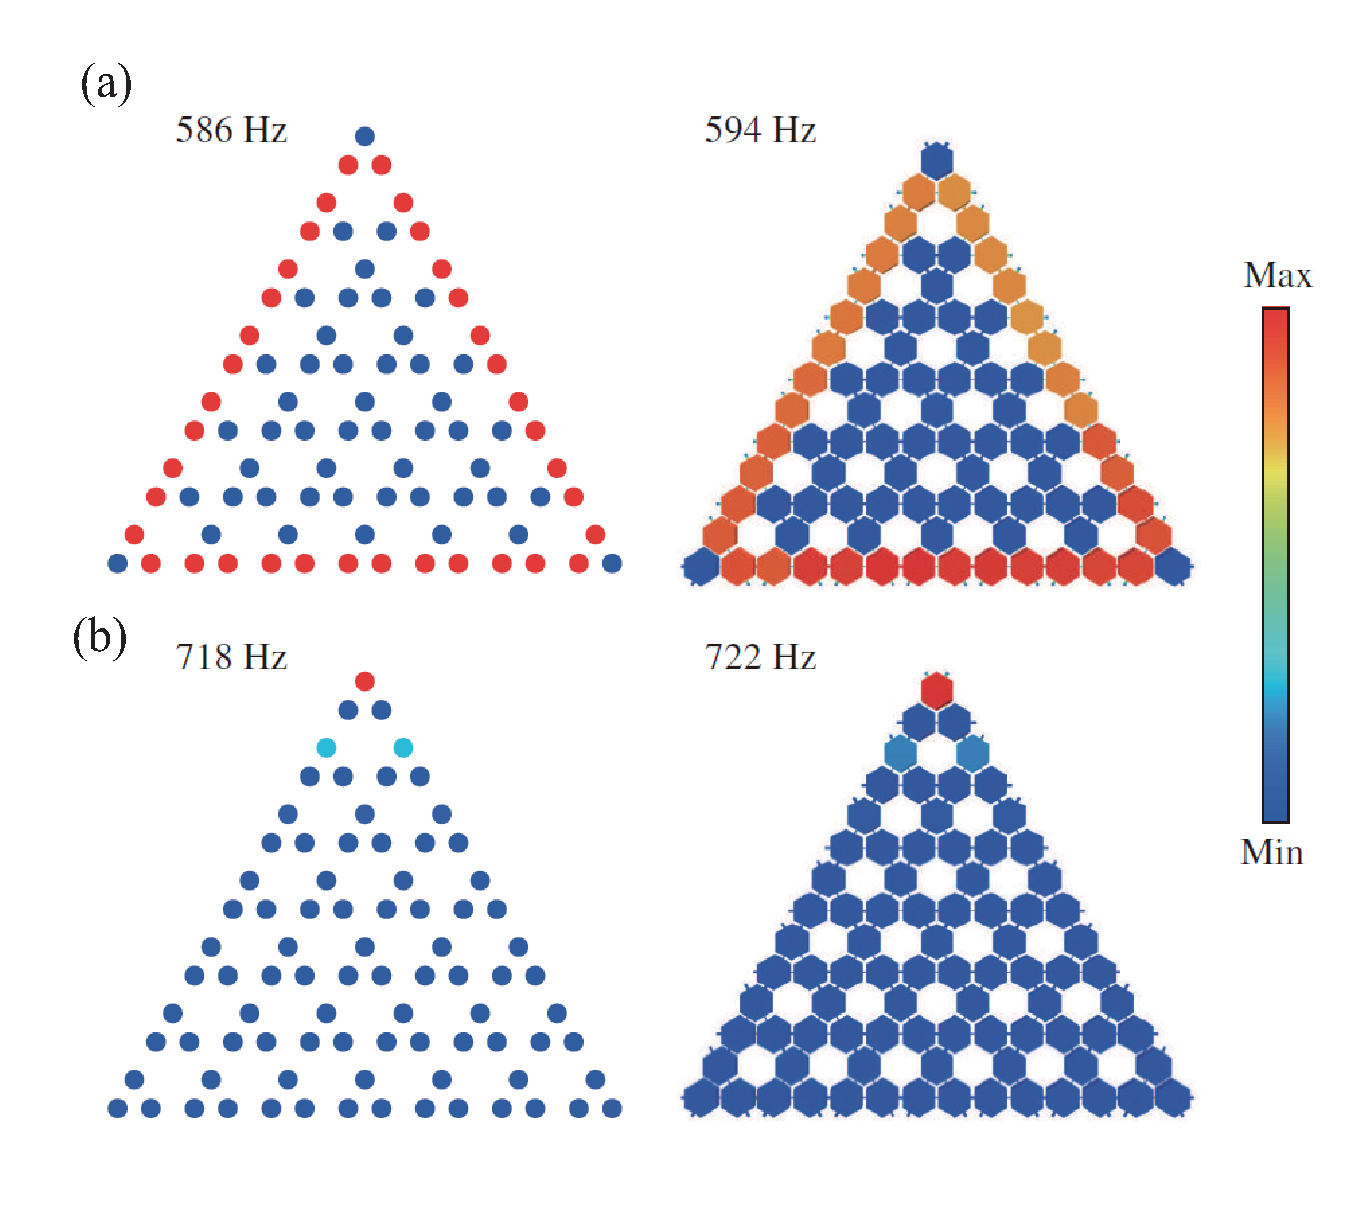
\includegraphics[width=1\textwidth]{images/fig3-12.eps} 
  \caption{具有软边界的边界态和角态的理论结果与模拟结果: (a) 拓扑边界态的声压场分布。(b) 拓扑角态的声压场分布。左侧面板是理论结果,右侧面板是模拟结果。}
  \label{fig_3_12}
\end{figure}

\section{小结}
总之,我们提出了一种基于具有Kagome晶格的声学拓扑绝缘体来获得严格哈密顿量的通用方法,这揭示了声学系统中的高阶拓扑。值得一提的是,我们证明了封闭的平凡材料对于拓扑态并非必要,这拓宽了设计拓扑绝缘体声学类似物的范围。通过这种方法,很好地阐述了哈密顿量的对角项与有限结构的边界条件之间的关系,这会对封闭系统的拓扑态产生显著影响。我们证明了只有软边界恰好与电子系统中对角项为零的哈密顿量相符合,其中存在“零能”角态。关键的是,这种方法反过来可以构建具有特定拓扑现象的所需哈密顿量,进而直接设计精确的物理结构。同时,我们注意到这种方法可以很容易地扩展到更高维度。我们的工作有助于理解声学系统中的拓扑,有望为定量设计拓扑声学材料提供一个平台。